\ylDisplay{Peeglid} % Ülesande nimi
{Autor} % Autor
{lõppvoor} % Voor
{2010} % Aasta
{P 1} % Ülesande nr.
{1} % Raskustase
{
% Teema: Valgusõpetus
\ifStatement
Kaks paralleelset tasapeeglit on paigutatud vastamisi vahekaugusega $d = 3$ m. Peeglite vahel seisev inimene näeb endast mitut kujutist, millest osa paikneb tema poole seljaga ja osa näoga. Kui kaugel paiknevad teineteisest kaks samas suunas vaatavat järjestikust kujutist?
\fi
\ifHint
Samapidised on inimese kujutis peeglis ja selle kujutise teine kujutis.
\fi
\ifSolution
\begin{center}
	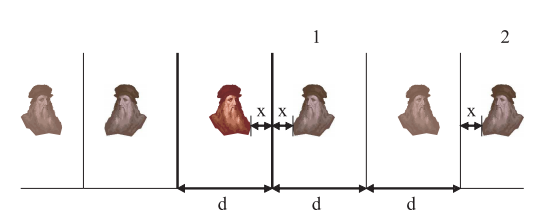
\includegraphics[width=0.5\linewidth]{2010-v3p-01-lah.PNG}
\end{center}
Joonisel on vaatleja ja reaalsed peeglid kujutatud tumedamalt. Kõik peeglite kujutised on üksteisest kaugusel $d$. Kui vaatleja asub enda ees seisvast peeglist kaugusel $x$, siis on tema esimese kujutise kaugus sellest peeglist samuti $x$. Teise samas suunas vaatava kujutise kaugus sellest peeglist on $2d + x$. Seetõttu on kujutiste omavaheline kaugus $2d + x - x = 2d = 6$ m.
\fi
}
